% Figures/pendulum.tex
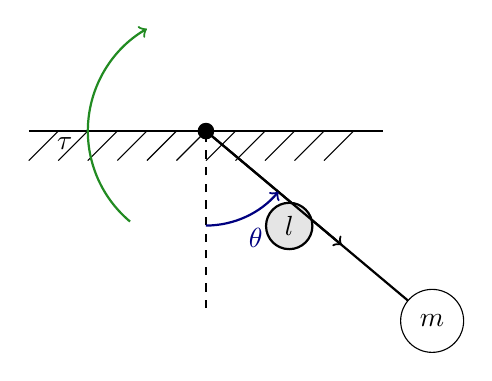
\begin{tikzpicture}[scale=1.5]
    % Support
    \draw[thick] (-1.5, 0) -- (1.5, 0);
    \foreach \i in {-1.25,-1,...,1.25} {
            \draw (\i, 0) -- (\i-0.25, -0.25);
        }

    % Pivot
    \fill[black] (0,0) circle (2pt);

    % Pendulum
    \def\angle{-40}
    \def\len{2.5}
    \draw[thick] (0,0) -- (\angle:\len) node[circle, draw, fill=gray!20, midway, left=2pt] {$l$};

    % Mass
    \node[circle, draw, fill=white, minimum size=0.8cm] (mass) at (\angle:\len) {$m$};

    % Angle
    \draw[->, dashed] (0,-1.5) -- (0,0);
    \draw[->, thick] (0,0) -- (\angle:1.5);
    \draw[->, thick, ForestGreen] (\angle-90:1) arc (\angle-90:\angle-200:1);
    \node at (\angle-135:1.2) {$\tau$};

    % Angle arc
    \draw[->, thick, NavyBlue] (0,0) ++(-90:0.8) arc (-90:\angle:0.8);
    \node[NavyBlue] at (-65:1) {$\theta$};
\end{tikzpicture}